% This is text associated with the open textbook "Open Electromagnetics"
% See immediately below for author, date
% This work is licensed under the Creative Commons Attribution-ShareAlike 4.0 International License. (CC BY-SA 4.0) 
% To view a copy of the license, visit http://creativecommons.org/licenses/by-sa/4.0/

%ORB TITLE Plane Waves at Oblique Incidence on a Planar Boundary: TE Case
%ORB AUTHOR 0        # S.W. Ellingson, Virginia Tech (ellingson@vt.edu)
%ORB DATE 20191124   # yyyymmdd
%ORB ABSTRACT 

\label{m0167_Oblique_Incidence_TE} % <-- Must match name of this file and module directory name.  Don't mess with this!
\index{transverse electric|(}

In this section, we consider the problem of reflection and transmission from a planar boundary between semi-infinite media for a transverse electric (TE) uniform plane wave.
Before attempting this section, a review of
Sections~\ref{m0161_Waves_at_Planar_Boundary} (``Plane Waves at Normal Incidence on a Planar Boundary Between Lossless Media'') and
\ref{m0166_Decomposition_into_TE_and_TM} (``Decomposition of a Wave into TE and TM Components'') is recommended.
Also, note that this section has much in common with Section~\ref{m0164_Oblique_Incidence_TM} (``Plane Waves at Oblique Incidence on a Planar Boundary: TM Case''), although it is recommended to attempt the TE case first.

The TE case is illustrated in Figure~\ref{m0167_fObliqueTE}.
%
\begin{figure}[b!]
\begin{center}
\pdftooltip{{  % note double braces
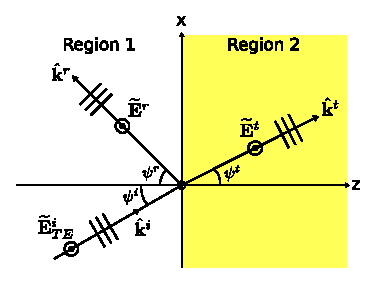
\includegraphics[width=0.8\columnwidth]{modules/m0167_fObliqueTE.eps} 
% https://commons.wikimedia.org/wiki/File:TE-polarized_upw_incident_on_planar_boundary.svg
}}{For a z-x coordinate system, region 1 is all negative z and region 2 is all positive z. A transverse electric wave is obliquely incident on the planar boundary. The reflected plane in region 1 for positive x. }
\end{center}
\centerline{\scriptsize 
\copyright~\hyperref[m0167_fObliqueTE_Credit]{C.\ Wang} 
\href{https://creativecommons.org/licenses/by-sa/4.0/}{CC BY-SA 4.0} 
} 
\caption{
\label{m0167_fObliqueTE}
A TE uniform plane wave obliquely incident on the planar boundary between two semi-infinite material regions.
}
\end{figure}
%
The boundary between the two semi-infinite and lossless regions is located at the $z=0$ plane.
The wave is incident from Region~1. 
The electric field intensity $\widetilde{\bf E}^i_{TE}$ of this wave is given by
%
\begin{equation}
\widetilde{\bf E}^i_{TE}({\bf r}) = \hat{\bf y} E^i_{TE} e^{-j{\bf k}^i\cdot{\bf r}}
\label{m0167_eEi}
\end{equation}
%
In this expression, ${\bf r}$ is the position at which $\widetilde{\bf E}^i_{TE}$ is evaluated, and 
%
\begin{equation}
{\bf k}^i = \hat{\bf k}^i \beta_1
\end{equation}
%
where
$\hat{\bf k}^i$ is the unit vector indicating the direction of propagation and
$\beta_1=\omega\sqrt{\mu_1 \epsilon_1}$ is the phase propagation constant in Region~1. 
$\widetilde{\bf E}^i_{TE}$ serves as the ``stimulus'' in this problem, so all other contributions to the total field will be expressed in terms of quantities appearing in Equation~\ref{m0167_eEi}.

The presence of reflected and transmitted uniform plane waves is inferred from our experience with the normal incidence scenario (Section~\ref{m0161_Waves_at_Planar_Boundary}).
There, as here, the symmetry of the problem indicates that the reflected and transmitted components of the electric field will have the same polarization as that of the incident electric field.  This is because there is nothing present in the problem that could account for a change in polarization.
Thus, the reflected and transmitted fields will also be TE.
Therefore, we postulate the following expression for the reflected wave:
%
\begin{equation}
\widetilde{\bf E}^r({\bf r}) = \hat{\bf y} B e^{-j{\bf k}^r\cdot{\bf r}}
\label{m0167_eEr}
\end{equation}
%
where $B$ is an unknown, possibly complex-valued constant to be determined and
%
\begin{equation}
{\bf k}^r = \hat{\bf k}^r \beta_1
\end{equation}
%
indicates the direction of propagation, which is also currently unknown.

Similarly, we postulate the following expression for the transmitted wave:
%
\begin{equation}
\widetilde{\bf E}^t({\bf r}) = \hat{\bf y} C e^{-j{\bf k}^t\cdot{\bf r}}
\label{m0167_eEt}
\end{equation}
%
where $C$ is an unknown, possibly complex-valued constant to be determined;
%
\begin{equation}
{\bf k}^t = \hat{\bf k}^t \beta_2
\end{equation}
%
where
$\hat{\bf k}^t$ is the unit vector indicating the direction of propagation; and
$\beta_2=\omega\sqrt{\mu_2 \epsilon_2}$ is the phase propagation constant in Region~2.

At this point, the unknowns in this problem are the constants $B$ and $C$, as well as the directions $\hat{\bf k}^r$ and $\hat{\bf k}^t$.  
We may establish a relationship between $E^i_{TE}$, $B$, and $C$ by application of boundary conditions at $z=0$.  
First, recall that the tangential component of the total electric field intensity must be continuous across material boundaries.
To apply this boundary condition, let us define $\widetilde{\bf E}_1$ and $\widetilde{\bf E}_2$ to be the total electric fields in Regions~1 and 2, respectively.
The total field in Region~1 is the sum of incident and reflected fields, so
%
\begin{equation}
\widetilde{\bf E}_1({\bf r}) = \widetilde{\bf E}^i_{TE}({\bf r}) + \widetilde{\bf E}^r({\bf r})
\end{equation}
%
The total field in Region~2 is simply
%
\begin{equation}
\widetilde{\bf E}_2({\bf r}) = \widetilde{\bf E}^t({\bf r})
\end{equation}
%
Next, note that all electric field components are already tangent to the boundary.
Thus, continuity of the tangential component of the electric field across the boundary requires $\widetilde{\bf E}_1(0)=\widetilde{\bf E}_2(0)$, and therefore
%
\begin{equation}
\widetilde{\bf E}^i_{TE}({\bf r}_0) + \widetilde{\bf E}^r({\bf r}_0)  = \widetilde{\bf E}^t({\bf r}_0) 
\end{equation}
%
where ${\bf r}={\bf r}_0\triangleq\hat{\bf x}x+\hat{\bf y}y$ since $z=0$ on the boundary.
Now employing Equations~\ref{m0167_eEi}, \ref{m0167_eEr}, and \ref{m0167_eEt}, we obtain:
%
\begin{equation}
\hat{\bf y}E^i_{TE}e^{-j{\bf k}^i\cdot{\bf r}_0} + 
\hat{\bf y}B         e^{-j{\bf k}^r\cdot{\bf r}_0} = 
\hat{\bf y}C         e^{-j{\bf k}^t\cdot{\bf r}_0}
\label{m0167_eBCE}
\end{equation}
%
Dropping the vector ($\hat{\bf y}$) since it is the same in each term, we obtain:
%
\begin{equation}
E^i_{TE}e^{-j{\bf k}^i\cdot{\bf r}_0} + 
B         e^{-j{\bf k}^r\cdot{\bf r}_0} = 
C         e^{-j{\bf k}^t\cdot{\bf r}_0}
\label{m0167_eBCE2}
\end{equation}

For Equation~\ref{m0167_eBCE2} to be true at every point ${\bf r}_0$ on the boundary, it must be true that
%
\begin{equation}
{\bf k}^i\cdot{\bf r}_0 = {\bf k}^r\cdot{\bf r}_0 = {\bf k}^t\cdot{\bf r}_0
\label{m0167_eSL}
\end{equation}
%
Essentially, we are requiring the phases of each field in Regions~1 and 2 to be matched at every point along the boundary.
Any other choice will result in a violation of boundary conditions at some point along the boundary.
This phase matching criterion will determine the directions of propagation of the reflected and transmitted fields, which we shall do later.  

First, let us use the phase matching criterion to complete the solution for the coefficients $B$ and $C$. 
Enforcing Equation~\ref{m0167_eSL}, we observe that Equation~\ref{m0167_eBCE2} reduces to:
%
\begin{equation}
E^i_{TE} + B = C 
\label{m0167_eBCE3}
\end{equation}

A second equation is needed since we currently have only one equation (Equation~\ref{m0167_eBCE3}) and two unknowns ($B$ and $C$).  
The second equation is obtained by applying the appropriate boundary conditions to the magnetic field.
The magnetic field associated with each of the electric field components is identified in Figure~\ref{m0167_fObliqueTE-H}.
%
\begin{figure}
\begin{center}
\pdftooltip{{  % note double braces
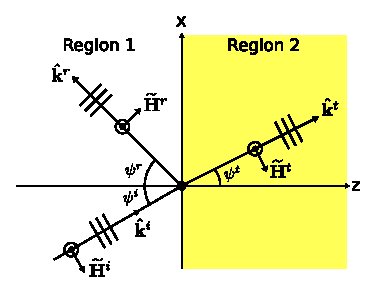
\includegraphics[width=0.8\columnwidth]{modules/m0167_fObliqueTE-H.eps} 
% https://commons.wikimedia.org/wiki/File:Incident_reflected_and_transmitted_magnetic_field_components.svg
}}{Associated magnetic field intensity components.}
\end{center}
\centerline{\scriptsize 
\copyright~\hyperref[m0167_fObliqueTE-H_Credit]{C.\ Wang} 
\href{https://creativecommons.org/licenses/by-sa/4.0/}{CC BY-SA 4.0} 
} 
\caption{
\label{m0167_fObliqueTE-H}
Incident, reflected, and transmitted magnetic field components associated with the TE electric field components shown in Figure~\ref{m0167_fObliqueTE}.
}
\end{figure}
%
Note the orientations of the magnetic field vectors may be confirmed using the \emph{plane wave relationships}: 
\index{plane wave relationships}
Specifically, the cross product of the electric and magnetic fields should point in the direction of propagation.
Expressions for each of the magnetic field components is determined formally below.

From the plane wave relationships, we determine that the incident magnetic field intensity is
%
\begin{equation}
\widetilde{\bf H}^i({\bf r}) = \frac{1}{\eta_1} \hat{\bf k}^i \times \widetilde{\bf E}^i_{TE}              
\label{m0167_eHi}
\end{equation}
%
where $\eta_1=\sqrt{\mu_1 / \epsilon_1}$ is the wave impedance in Region~1.  
%
To make progress requires that we express $\hat{\bf k}^i$ in the global fixed coordinate system.  Here it is:
%
\begin{equation}
\hat{\bf k}^i = \hat{\bf x}\sin\psi^i + \hat{\bf z}\cos\psi^i 
\end{equation}
%
Thus:
%
\begin{equation}
\widetilde{\bf H}^i({\bf r}) = \left( \hat{\bf z}\sin\psi^i - \hat{\bf x}\cos\psi^i \right) \frac{E^i_{TE}}{\eta_1}  e^{-j{\bf k}^i\cdot{\bf r}}          
\label{m0167_eHi2}
\end{equation}
%
Similarly, we determine that the reflected magnetic field has the form:
%
\begin{equation}
\widetilde{\bf H}^r({\bf r}) = \frac{1}{\eta_1} \hat{\bf k}^r \times \widetilde{\bf E}^r              
\label{m0167_eHr}
\end{equation}
%
In the global coordinate system:
%
\begin{equation}
\hat{\bf k}^r = \hat{\bf x}\sin\psi^r - \hat{\bf z}\cos\psi^r 
\label{m0167_ehkr}
\end{equation}
%
Thus:
%
\begin{equation}
\widetilde{\bf H}^r({\bf r}) = \left( \hat{\bf z}\sin\psi^r + \hat{\bf x}\cos\psi^r \right) \frac{B}{\eta_1}  e^{-j{\bf k}^r\cdot{\bf r}}          
\label{m0167_eHr2}
\end{equation}
%
The transmitted magnetic field has the form:
%
\begin{equation}
\widetilde{\bf H}^t({\bf r}) = \frac{1}{\eta_2} \hat{\bf k}^t \times \widetilde{\bf E}^t              
\label{m0167_eHt}
\end{equation}
%
In the global coordinate system:
%
\begin{equation}
\hat{\bf k}^t = \hat{\bf x}\sin\psi^t + \hat{\bf z}\cos\psi^t 
\label{m0167_ehkt}
\end{equation}
%
Thus:
%
\begin{equation}
\widetilde{\bf H}^t({\bf r}) = \left( \hat{\bf z}\sin\psi^t - \hat{\bf x}\cos\psi^t \right) \frac{C}{\eta_2}  e^{-j{\bf k}^t\cdot{\bf r}}          
\label{m0167_eHt2}
\end{equation}
%
The total magnetic field in Region~1 is the sum of incident and reflected fields, so
%
\begin{equation}
\widetilde{\bf H}_1({\bf r}) = \widetilde{\bf H}^i({\bf r}) + \widetilde{\bf H}^r({\bf r})
\end{equation}
%
The magnetic field in Region~2 is simply
%
\begin{equation}
\widetilde{\bf H}_2({\bf r}) = \widetilde{\bf H}^t({\bf r})
\end{equation}
%
Since there is no current on the boundary, the tangential component of the total magnetic field intensity must be continuous across the boundary.
Expressed in terms of the quantities already established, this boundary condition requires:
%
\begin{equation}
\hat{\bf x}\cdot\widetilde{\bf H}^i({\bf r}_0) + \hat{\bf x}\cdot\widetilde{\bf H}^r({\bf r}_0)  = \hat{\bf x}\cdot\widetilde{\bf H}^t({\bf r}_0) 
\end{equation}
%
where ``$\hat{\bf x}\cdot$'' selects the component of the magnetic field that is tangent to the boundary.
Evaluating this expression, we obtain:
%
\begin{flalign}
  &-\left(\cos\psi^i\right)\frac{E^i_{TE}}{\eta_1}e^{-j{\bf k}^i\cdot{\bf r}_0} \nonumber \\
  &+\left(\cos\psi^r\right)\frac{B}{\eta_1}e^{-j{\bf k}^r\cdot{\bf r}_0} \nonumber \\
= &-\left(\cos\psi^t\right)\frac{C}{\eta_2}e^{-j{\bf k}^t\cdot{\bf r}_0} 
\end{flalign}
%
Now employing the phase matching condition expressed in Equation~\ref{m0167_eSL}, we find:
%
\begin{flalign}
  &-\left(\cos\psi^i\right)\frac{E^i_{TE}}{\eta_1} \nonumber \\
  &+\left(\cos\psi^r\right)\frac{B}{\eta_1} \nonumber \\
= &-\left(\cos\psi^t\right)\frac{C}{\eta_2} 
\label{m0167_eBCH3}
\end{flalign}

Equations~\ref{m0167_eBCE3} and \ref{m0167_eBCH3} comprise a linear system of equations with unknowns $B$ and $C$.
This system of equations is easily solved for $B$ as follows.
First, use Equation~\ref{m0167_eBCE3} to eliminate $C$ in Equation~\ref{m0167_eBCH3}.
The result is: 
%
\begin{flalign}
  &-\left(\cos\psi^i\right)\frac{E^i_{TE}}{\eta_1} \nonumber \\
  &+\left(\cos\psi^r\right)\frac{B}{\eta_1} \nonumber \\
= &-\left(\cos\psi^t\right)\frac{E^i_{TE}+B}{\eta_2} 
\end{flalign}
%
Solving this equation for $B$, we obtain:
%
\begin{equation}
B = \frac{\eta_2\cos\psi^i-\eta_1\cos\psi^t}{\eta_2\cos\psi^r+\eta_1\cos\psi^t} ~ E^i_{TE}
\end{equation}
%
We can express this result as a reflection coefficient as follows:
%
\begin{equation}
B = \Gamma_{TE} E^i_{TE} 
\end{equation}
%
where
%
\begin{equation}
\Gamma_{TE} \triangleq \frac{\eta_2\cos\psi^i-\eta_1\cos\psi^t}{\eta_2\cos\psi^r+\eta_1\cos\psi^t}
\label{m0167_eGTE}
\end{equation}
%
It is worth noting that Equation~\ref{m0167_eGTE} becomes the reflection coefficient for normal (TEM) incidence when $\psi^i=\psi^r=\psi^t=0$, as expected.

Returning to Equation~\ref{m0167_eBCE3}, we now find
%
\begin{equation}
C = \left(1+\Gamma_{TE}\right) E^i_{TE} 
\end{equation}

Let us now summarize the solution.  Given the TE electric field intensity expressed in Equation~\ref{m0167_eEi}, we find:
%
\begin{equation}
\boxed{ \widetilde{\bf E}^r({\bf r}) = \hat{\bf y}\Gamma_{TE}E^i_{TE}e^{-j{\bf k}^r\cdot {\bf r}} }
\end{equation}
%
\begin{equation}
\boxed{ \widetilde{\bf E}^t({\bf r}) = \hat{\bf y}\left(1+\Gamma_{TE}\right)E^i_{TE}e^{-j{\bf k}^t\cdot {\bf r}} } 
\end{equation}
%
This solution is complete except that we have not yet determined 
$\hat{\bf k}^r$, which is now completely determined by $\psi^r$ via Equation~\ref{m0167_ehkr}, and
$\hat{\bf k}^t$, which is now completely determined by $\psi^t$ via Equation~\ref{m0167_ehkt}.
In other words, we have not yet determined the directions of propagation 
$\psi^r$ for the reflected wave and
$\psi^t$ for the transmitted wave.
However, $\psi^r$ and $\psi^i$ can be found using Equation~\ref{m0167_eSL}.
Here we shall simply state the result, and in Section~\ref{m0168_Angles_of_Reflection_and_Refraction} we shall perform this part of the derivation in detail and with greater attention to the implications.
One finds:
%
\begin{equation}
\psi^r = \psi^i
\label{m0167_epsir}
\end{equation}
%
and
%
\begin{equation}
\psi^t = \arcsin\left(\frac{\beta_1}{\beta_2}\sin\psi^i\right)
\label{m0167_epsit}
\end{equation}
%
Equation~\ref{m0167_epsir} is the unsurprising result that angle of reflection equals angle of incidence.
Equation~\ref{m0167_epsit} -- addressing angle of transmission -- is a bit more intriguing.  Astute readers may notice that there is something fishy about this equation: 
It seems possible for the argument of $\arcsin$ to be greater than one.
This oddity is addressed in Section~\ref{m0168_Angles_of_Reflection_and_Refraction}.

Finally, note that Equation~\ref{m0167_epsir} allows us to eliminate $\psi^r$ from Equation~\ref{m0167_eGTE}, yielding:
%
\begin{equation}
\boxed{
\Gamma_{TE} = \frac{\eta_2\cos\psi^i-\eta_1\cos\psi^t}{\eta_2\cos\psi^i+\eta_1\cos\psi^t}
}
\label{m0167_eGTE2}
\end{equation}
%
Thus, we obtain what is perhaps the most important finding of this section:
%%%%%%%%%%%%%%%%%%%%%%%%%%%%%%%%%%%%%%%%%%%%%%%
%ORB HIGHLIGHT
\begin{mdframed}[backgroundcolor=yellow!20,nobreak=true] 
The electric field reflection coefficient for oblique TE incidence, $\Gamma_{TE}$, is given by Equation~\ref{m0167_eGTE2}.
\end{mdframed}
%%%%%%%%%%%%%%%%%%%%%%%%%%%%%%%%%%%%%%%%%%%%%%%
The following example demonstrates the utility of this result.

%%%%%%%%%%%%%%%%%%%%%%%%%%%%%%%%%%%%%%%%%%%%%%%
%ORB EXAMPLE
~\\ \begin{example} 
\label{m0167_exTERC}
\begin{mdframed}[backgroundcolor=brown!20,linecolor=brown!20]\raggedright
Power transmission at an air-to-glass interface (TE case).
\\~\\
Figure~\ref{m0167_fGlassExample} illustrates a TE plane wave incident from air onto the planar boundary with glass.
The glass exhibits relative permittivity of 2.1.  
Determine the power reflected and transmitted relative to power incident on the boundary.\\
~\\

\noindent
{\bf Solution.}
The power reflected relative to power incident is $\left|\Gamma_{TE}\right|^2$ whereas
the power transmitted relative to power incident is $1-\left|\Gamma_{TE}\right|^2$.
$\Gamma_{TE}$ may be calculated using Equation~\ref{m0167_eGTE2}.
Calculating the quantities that enter into this expression:
%
\begin{equation} 
\eta_1 \approx \eta_0 \cong 376.7~\Omega ~~ \mbox{(air)} 
\end{equation}
%
%
\begin{equation} 
\eta_2 \approx \frac{\eta_0}{\sqrt{2.1}} \cong 260.0~\Omega ~~ \mbox{(glass)} 
\end{equation}
%
\begin{equation}
\psi^i = 30^{\circ} 
\end{equation}
Note
\begin{equation}
\frac{\beta_1}{\beta_2} \approx \frac{\omega\sqrt{\mu_0\epsilon_0}}{\omega\sqrt{\mu_0\cdot2.1\epsilon_0}} \cong 0.690 
\end{equation}
%
so
\begin{equation}
\psi^t = \arcsin\left(\frac{\beta_1}{\beta_2}\sin\psi^i\right) \cong 20.2^{\circ} 
\end{equation}
%
Now substituting these values into Equation~\ref{m0167_eGTE2}, we obtain
%
\begin{equation}
\Gamma_{TE} \cong -0.2220 
\end{equation}
%
Subsequently, the fraction of power reflected relative to power incident is $\left|\Gamma_{TE}\right|^2\cong 0.049$; i.e., about \underline{4.9\%}.
$1-\left|\Gamma_{TE}\right|^2\cong$ \underline{95.1\%} of the power is transmitted into the glass.
\end{mdframed}
%
\begin{figure}
\begin{center}
\pdftooltip{{  % note double braces
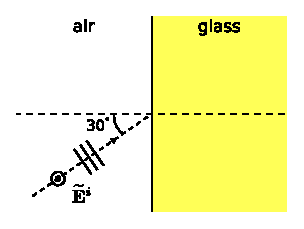
\includegraphics[width=0.8\columnwidth]{modules/m0167_fGlassExample.eps} 
% https://commons.wikimedia.org/wiki/File:TE-polarized_upw_incident_from_air_to_glass.svg
}}{Capital E tilde superscript i out of page. Plane wave is incident at a 30 degree angle from the horizon.}
\end{center}
\centerline{\scriptsize 
\copyright~\hyperref[m0167_fGlassExample_Credit]{C.\ Wang} 
\href{https://creativecommons.org/licenses/by-sa/4.0/}{CC BY-SA 4.0} 
} 
\caption{
\label{m0167_fGlassExample}
A TE uniform plane wave incident from air to glass.
}
\end{figure}
\end{example}
%%%%%%%%%%%%%%%%%%%%%%%%%%%%%%%%%%%%%%%%%%%%%%%

\index{transverse electric|)}


